\documentclass[a4paper,
  twoside, % two have to sided mode (odd and even page numbers)
  headlines=2.1 % number of lines in the heading, increase if you want more
  ]{scrartcl}

% Packages
\usepackage[english]{babel}
\usepackage[utf8]{inputenc}
\usepackage[T1]{fontenc}
\usepackage{siunitx}
\usepackage{lipsum}
\usepackage[left=2.5cm,right=2.5cm,top=2.5cm,bottom=2.5cm]{geometry}
\usepackage[onehalfspacing]{setspace}
\usepackage{lmodern}
\usepackage[automark,headsepline]{scrlayer-scrpage}
\usepackage[numbers]{natbib}
\usepackage{csquotes}
\usepackage{textcomp}
\usepackage{hyperref}
\usepackage{graphicx}
\usepackage{cleveref}

% Commands
\setlength{\parskip}{1em}
\setlength\parindent{0pt}

\newcommand{\yourname}{Marc Johannes Aslan \and Thomas Kötzner}
\newcommand{\headingname}{Marc Johannes Aslan, Thomas Kötzner}
\newcommand{\lecture}{MST Technologies and Processes, Assignments, course winter semester 2018/2019}
\author{\yourname}
\title{\lecture}

\pagestyle{scrheadings}
\setkomafont{pagehead}{\normalfont}
\lohead{\lecture\\\today}
\lehead{\lecture\\\today}
\rohead{\\}
\rehead{\\}

\title{MST Technolgies and Processes}
\subtitle{Assignement \#2: High aspect ratio MEMS}
\date{\today}
\author{Thomas Kötzner, Marc Johannes Aslan}
\date{January 2019}





\begin{document}

\maketitle

\section{Task}
The aim of this assignement is to introduce and describe high aspect ratio MEMS. Furthermore, typlical applications of high aspect ratio MEMS are presented. Finally, methods are shown with which high aspect ratio MEMS structures can be produced. This involves methods for different materials such as metals, polymers and semiconductors.

\section{Introduction}
As Richard Feynman already stated in his famous lecture \enquote{There's plenty of room at the bottom} in 1960, that there should be a field, in which it is possible to manipulate matter on an atomic scale. \cite{feynman2012} With these techniques, it should be possible to build nanoscale machines or sensors. Nearly 60 years later, this field is known as micro systems technology, where such tiny structures are typical and used for different applications. To achieve manufacturing such devices, there are plenty different technologies. For each of them, there are certain advantages and disadvantages, which are also dependent of the different applications. In most cases it is typical to use high aspect ratio micro structure technology (HARMST). HARMST devices are required for a number of common applications like sensors. The improvement in plasma techniques made the fabrication of such structures possible. 


\section{High aspect ratio micro structure technolgy}
Aspect ratio is described as ratio between the depth or rather height and the minimal lateral expansion of the structure. In some publications high aspect ratio is defined bigger than 10:1, in others 50:1. \cite{mcnie2000} One advantage of high aspect ratio is the increased flexibility in 3 dimensions. It is possible to build structures of different shapes and varying heights or widths. This is often used for applications with high packaging density, using the height rather the width reduces the needed space on the substrate.\cite{mcnie2000} Due to the increased height, which offers bigger areas, it is possible to increase the capacitance of the structures, which is needed in many applications. Bigger capacities are required for applications with lower driving voltages. Also, the sensitivity is improved, e.g. in applications where micro mechanical motions should be detected, because it is easier to detect changes in bigger capacities. \cite{pang2001} For applications in critical areas like medical technology or automotive, high aspect ratio provides high security. It prevents e.g. cross axis coupling or immunity to high frequency and high amplitude parasitic effects. \cite{mcnie2000,NXP2009}. Furthermore, high aspect ratio provides an exceptional signal-to-noise ratio and over-damped mechanical response. \cite{NXP2009} Another characteristic of high aspect ratio is the possibility to build thick high mass elements. Those are often used to increase mechanical stability, which leads to more robustness. Also, released features of MEMS can be formed, where the stress due to bending is reduced. \cite{mcnie2000, pang2001, hutchison2010} Typical production processes for these structures are \enquote{Deep Reactive Ion Etching} (DRIE), \enquote{Lithographie, Galvanik und Abformung} (LIGA) and \enquote{Single Crystal Reactive Etching And Metallization} (SCREAM). According to the process, higher ratios could be reached and several materials are editable. Nevertheless, it must be said, that those processes are more complex and expensive than techniques like conventional dry etching or lithography. On top of that, the planning effort to design these structures is bigger, because it is necessary to take care of effects like the critical aspect ratio. Important parameters are e.g. are the own weight of the structures, inertia, angles of released features to the substrate and shear effects.

%Johannes 1 2 kleine Bilder 1 Seite -> 3.5
\section{Applications}
- Microinertial Sensors

- Nanotubes

\section{Fabrication methods}
This sections describes different processes and for which materials they are used

% Johannes 0.24
\subsection{Metals}
\subsubsection{LIGA}
\cite{BECKER198635}

%Johannes 0.25 -> 4
\subsection{Polymers}

% Thomas 
\subsection{Semiconductor materials}
\subsubsection{Deep Reactive Ion Etching (DRIE) }
Deep Reative Ion Etching is an enhancement of reactive Ion Etching and was developed by Robert Bosch AG in 1990. This anisotropic process is the most common technique to produce an very high aspect ratio on silicon. An aspect ratio up to 50:1 is achievable. This aspect ratio is not as high like in the LIGA process, but the advantages of DIRE are cost savings and faster process time. Also the previously mentioned aspect ratio is high enough for the most applications, like  Microsystems and 3D-Integration of electrical circuits. It is possible to etch 20 \textmu m per minute, but usually the substrate is etched with a speed of 1-2 \textmu m per minute, to get more precision and less wave-like structures on the side walls of the etching channel. An simplified process discretion is shown in \cref{Schematic_drie}. First of all, what is not mentioned in the figure, a mask is attached to the substrate, which protects the areas which should not be etched. After that, the first etching step is performed with SF\textsubscript{6}. The echting gas is removed and CF\textsubscript{4} is lead to the substrates. The gas reacts in an isotropic process with the silicon and builds a protecting plasma-polymer-layer on the top of the whole substrate as seen in \cref{Schematic_drie} Phase 1. To etch the next step, the previously mentioned anisotropic etching process will be repeated. Because of the anisotropic characteristic the SF\textsubscript{6} is etching through the protection layer at the bottom into the substrate, while the walls are nearly untouched. The three phases are repeated until the desired depth is reached. A disadvantage of this process is the litigation. It has to be optimized for every single structure, to get vertical and smooth side walls\cite{menz2005paul}.

\begin{figure}[h]
	\centering
	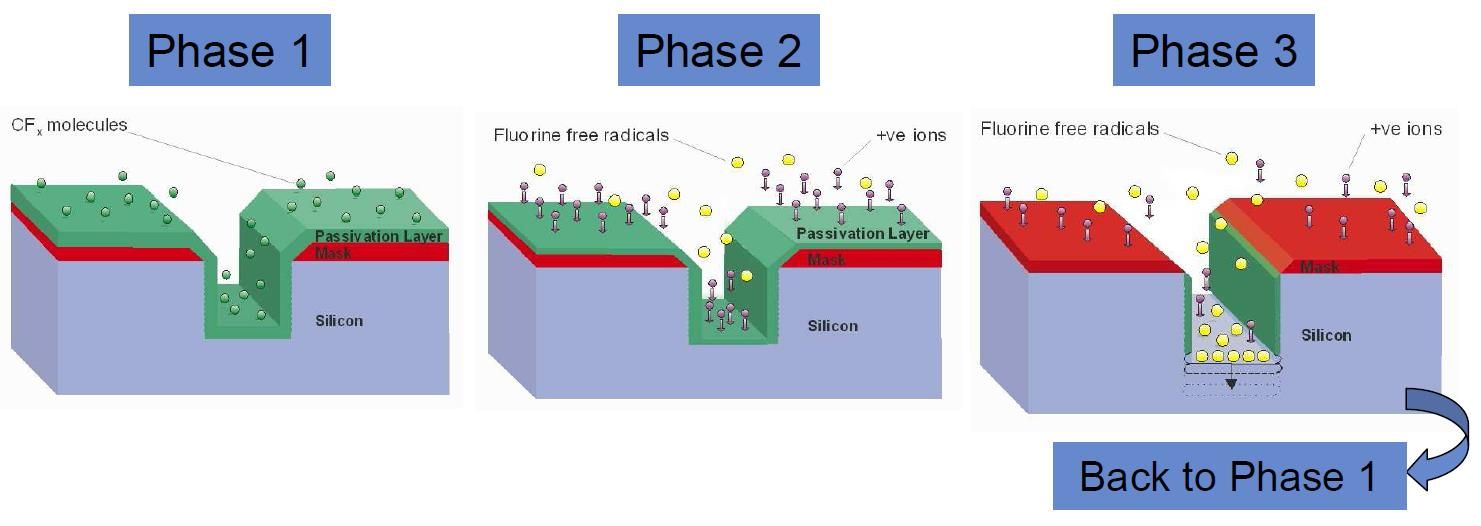
\includegraphics[width=\textwidth]{Graphics/DIRE/drie-schema_fraunhofer.jpg}
	\caption{Schematic representation of DRIE \cite{Fraunhofer2019}}
	\centering
	\label{Schematic_drie}
\end{figure} 
\subsubsection{UV-LIGA}
\subsubsection{Screem}

\section{Conclusion}

\clearpage
\bibliography{literature}
\bibliographystyle{IEEEtran}


\end{document}
